\section{\numb section 10. Internal details}

This section contains material intended to assist the developer in reading the source code
of \maniFEM.
It contains mainly drawings which document specific parts of \maniFEM.

Some components of {\maniFEM} (namely, those described in paragraphs \numb section 10.\numb parag 2,
\numb section 10.\numb parag 3 and \numb section 10.\numb parag 4) are written in two ``flavors'',
a pretty version which is easier
to read and an ugly version which should be slightly faster.
They are functionally equivalent.
The first one is recognizable by a {\codett tag::pretty}.
Reading both, side to side, should help the user understand the ``lower level'' programming style
in {\maniFEM}, so that later he or she may write new functions for extending and generalizing
{\maniFEM}.


\paragraph{\numb section 10.\numb parag 2. Building a chain of segments}

One of the simplest meshes is an open chain of segments.
\ Constructor \ {\codett Mesh ( tag::segment,...)}, declared in {\codett mesh.h} and defined in
{\codett global.cpp}, receives two vertices (a negative one and a positive one)
and the desired number of segments and builds the chain.
New vertices are built by using the constructor {\codett Cell ( tag::vertex )}.
Space coordinates of each new vertex are defined by interpolating the coordinates of the
two extremities of the chain.
New segments are built by means of constructor {\codett Cell ( tag::segment, A, B )},
where {\codett A} is a {\codett Cell::Negative::Vertex} and {\codett B} is a
{\codett Cell::Positive::Vertex}.

Note that the interpolation operation is a method belonging to {\codett space}
(an object belonging to the class {\codett Manifold}).
For an Euclidian manifold, this is just a convex combination of the values of the coordinates.
However, for other manifolds it may be a more complex operation.
For an implicit manifold, it involves a projection operation
(paragraphs \numb section 2.\numb parag 3 -- \numb section 2.\numb parag 9 show such examples).
For a manifold defined through an external parameter, the convex combination is performed on
the external parameter and then the space coordinates are computed accordingly (paragraphs
\dots show such a situation).


\paragraph{\numb section 10.\numb parag 3. Building a rectangular mesh}

Constructor {\codett Mesh::Mesh ( tag::rectangle,...)}, declared in {\codett mesh.h} and defined in
{\codett global.cpp}, builds a rectangular mesh from its
four sides (which are one-dimensional meshes, more precisely, open chains of segments).
No need to provide the number of divisions, the four sides have already their internal divisions.
Of course, opposite sides should have the same number of (segment) cells.

Paragraphs \numb section 1.\numb parag 3, \numb section 1.\numb parag 4 and many others (e.g.%
\ in section \numb section 2) show the use of this constructor.

Actually, the name {\codett rectangle} is misleading.
Perhaps a better name would be {\codett quadrangle} but even this is not general enough to
describe the constructor's ability to build curved patches like the ones shown in paragraphs
\numb section 1.\numb parag 1 or \numb section 2.\numb parag 6 -- \numb section 2.\numb parag 9.
Tags {\codett rectangle}, {\codett quadrangle} and {\codett quadrilateral} can be used
interchangeably.

Providing a {\codett tag::with\_triangles} makes the constructor cut each rectangle in halves;
results are shown in paragraphs \numb section 2.\numb parag 2 and \numb section 2.\numb parag 7.

{ \psfrag{A}{\special{ps: gsave 0 0 0.8 setrgbcolor}{\codett A}\special{ps: grestore}}
\psfrag{B}{\special{ps: gsave 0 0 0.8 setrgbcolor}{\codett B}\special{ps: grestore}}
\psfrag{C}{\special{ps: gsave 0 0 0.8 setrgbcolor}{\codett C}\special{ps: grestore}}
\psfrag{D}{\special{ps: gsave 0 0 0.8 setrgbcolor}{\codett D}\special{ps: grestore}}
\psfrag{south}{\special{ps: gsave 0 0 0.8 setrgbcolor}{\codett south}\special{ps: grestore}}
\psfrag{east}{\special{ps: gsave 0 0 0.8 setrgbcolor}{\codett east}\special{ps: grestore}}
\psfrag{north}{\special{ps: gsave 0 0 0.8 setrgbcolor}{\codett north}\special{ps: grestore}}
\psfrag{west}{\special{ps: gsave 0 0 0.8 setrgbcolor}{\codett west}\special{ps: grestore}}
\centerline{\includegraphics[width=80mm]{fig-rectangle.eps}} }

The coordinates of each new vertex are defined by interpolating the coordinates of four vertices
on the four given sides, as shown in the figure above.
The complicated formula for the coefficients (involving $ \alpha^3 $ and $ \beta^3 $) is there
to ensure a smooth transition for the distribution of inner vertices in the case of non-uniform
distribution along one or several sides.
Paragraphs \numb section 2.\numb parag 1, \numb section 2.\numb parag 8 and
\numb section 2.\numb parag 10 show examples where this is useful.

The remarks made in paragraph \numb section 10.\numb parag 2 about the interpolation operation
hold here.
Paragraph \numb section 2.\numb parag 6 shows an example where the interpolation operation
consists of a convex combination followed by a projection.
Paragraph \dots shows an example where the convex combination is done on an external parameter
rahter than on the coordinates themselves.


\paragraph{\numb section 10.\numb parag 4. Building a triangular mesh}

Building a triangular mesh involves an algorithm much alike the one for a rectangular mesh.
A noteworthy difference is that the interpolation operation involves now six vertices on
the boundary of the triangle, as shown in figure below.

{ \psfrag{A}{\special{ps: gsave 0 0 0.8 setrgbcolor}{\codett A}\special{ps: grestore}}
\psfrag{B}{\special{ps: gsave 0 0 0.8 setrgbcolor}{\codett B}\special{ps: grestore}}
\psfrag{C}{\special{ps: gsave 0 0 0.8 setrgbcolor}{\codett C}\special{ps: grestore}}
\psfrag{S}{\special{ps: gsave 0 0 0.8 setrgbcolor}{\codett S}\special{ps: grestore}}
\psfrag{P_AB}{\special{ps: gsave 0 0 0.8 setrgbcolor}{\codett P\_AB}\special{ps: grestore}}
\psfrag{Q_AB}{\special{ps: gsave 0 0 0.8 setrgbcolor}{\codett Q\_AB}\special{ps: grestore}}
\psfrag{P_BC}{\special{ps: gsave 0 0 0.8 setrgbcolor}{\codett P\_BC}\special{ps: grestore}}
\psfrag{Q_BC}{\special{ps: gsave 0 0 0.8 setrgbcolor}{\codett Q\_BC}\special{ps: grestore}}
\psfrag{P_CA}{\special{ps: gsave 0 0 0.8 setrgbcolor}{\codett P\_CA}\special{ps: grestore}}
\psfrag{Q_CA}{\special{ps: gsave 0 0 0.8 setrgbcolor}{\codett Q\_CA}\special{ps: grestore}}
\centerline{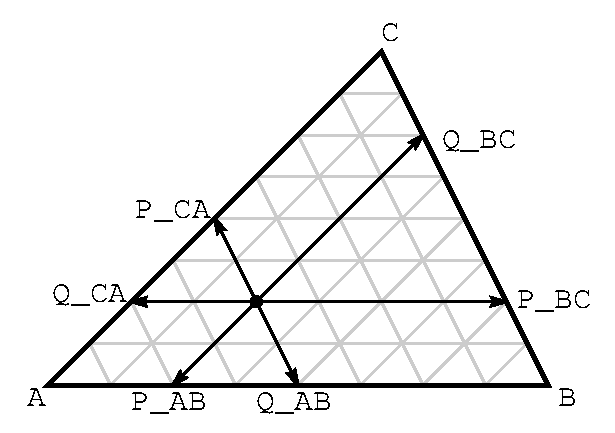
\includegraphics[width=75mm]{fig-triangle.eps}} }

The coefficients for the interpolation have simpler formulas when compared with the ones in the
constructor of a rectangle (presented in paragraph \numb section 10.\numb parag 3);
the fact that we interpolate from six vertices compensates that.

Examples are presented in paragraphs \numb section 1.\numb parag 4, \numb section 1.\numb parag 5
and \numb section 2.\numb parag 5
\vfil\eject

\paragraph{\numb section 10.\numb parag 5. Progressive mesh generation}

Constructor {\codett Mesh::Mesh ( tag::progressive, ... )}, declared in {\codett mesh.h} and defined
in {\codett progressive.cpp}, builds a mesh on a given manifold starting with almost nothing.
More precisely, it starts with the boundary of the future mesh, then it
moves this interface with small steps, building the mesh behind it like a spider.
Actually, if the manifold is compact (like the sphere or the torus) and we want to mesh all of it,
there will be no boundary.
In this case we can start the process by providing nothing more than the manifold itself.
Section \numb section 3 gives several examples.

This is a complex process, much more complex than building a regular mesh of rectangles
(as described in paragraph \numb section 10.\numb parag 3) or of triangles (as described
in paragraph \numb section 10.\numb parag 4).
The constructor delegates the job to the function {\codett progressive\_construct}.

The mesh must follow the shape of the manifold; this is achieved by {\codett project}ing
newly created vertices on the working manifold.

The initial interface may be disconnected.
Even if the initial interface is connected, it may become disconnected during the meshing
process, if it touches itself (paragraph \numb section 10.\numb parag 8 discusses this event).

Detecting such touching points requires evaluating the distance between many pairs of points.
This may become extremely time consuming, unless special care is taken to organize points
belonging to the interface in a hierarchy allowing one to eliminate many pairs of points
from the evaluation process.
Paragraph \numb section 9.\numb parag 15 describes this hierarchy.

The next few paragraphs describe specific parts of this process of progressive mesh generation.


\paragraph{\numb section 10.\numb parag 6. The normals}

The meshing process described in paragraph \numb section 10.\numb parag 5 uses a set of
normal vectors.
Each segment in the interface has associated to it
a vector tangent to the working manifold and normal to the interface (we can
think of the interface as a curve embedded in that two-dimensional manifold).
These normal vectors provide the sense in which we want the mesh to grow (to the left or to
the right of the interface), that is, they define the orientation of the manifold and of
the mesh under construction.
They are used when we create a new vertex in order to decide its placement.

Actually, at the beginning of the process only one segment has an associated normal vector.
{\ManiFEM} then propagates this normal vector to the neighbour segments, walking along
the current connected component of the interface.
This means that, if there are other connected components, they will have no normal vectors.
When the current connected component of the interface touches other connected components
(this event is discussed in paragraph \numb section 10.\numb parag 8), {\maniFEM}
% aproveita a oportunidade para ...
propagates the normal vectors to the new connected component.

Each time a new segment is added to the interface (this happens in situations described in
paragraphs \numb section 10.\numb parag 7 and \numb section 10.\numb parag 8),
the normal associated to the new segment must be computed (propagated from neighbour
segments).
\vfil\eject


\paragraph{\numb section 10.\numb parag 7. Filling triangles}

Perhaps the simplest part of the meshing process described in paragraph
\numb section 10.\numb parag 5 is just walking along the interface and adding new triangles.

A trivial case is when an angle is encountered which is close to $ 60^\circ $
(see figure below left).
Then we only have to fill the space with a new triangle.
Of course, before creating this new triangle a new segment {\codett AB} must be created
(no new vertex is needed).
Two old segments must be removed from the interface and the new one must be added.
Its normal must be computed (see paragraph \numb section 10.\numb parag 6).

{ \psfrag{A}{\special{ps: gsave 0 0 0.8 setrgbcolor}{\codett A}\special{ps: grestore}}
  \psfrag{B}{\special{ps: gsave 0 0 0.8 setrgbcolor}{\codett B}\special{ps: grestore}}
  \psfrag{P}{\special{ps: gsave 0 0 0.8 setrgbcolor}{\codett P}\special{ps: grestore}}
  \psfrag{point60}{\special{ps: gsave 0 0 0.8 setrgbcolor}
    {\codett point\_60}\special{ps: grestore}}
  \psfrag{point120}{\special{ps: gsave 0 0 0.8 setrgbcolor}
    {\codett point\_120}\special{ps: grestore}}
  \centerline{\includegraphics[width=45mm]{fill-angle-60.eps}
  \hskip5mm \includegraphics[width=45mm]{fill-angle-120.eps}} }

A more complicated situation is when an angle is encountered which is close to $ 120^\circ $
(see figure above right).
A new vertex {\codett P} is created; its position is defined based on the two normals
of the adjacent segments.
Two new segments {\codett AP} and {\codett BP} are created,
then two new triangles are created and added to the mesh under construction.
Two old segments are removed from the interface then {\codett AP} and {\codett BP} are added
to the interface (their normals must be computed).

Special situations must be dealt with.
For instance, if one or both neighbour angles are also close to $ 120^\circ $,
we must take more vertices into account when we place the newly created vertex {\codett P};
figure below shows such situations.

  \centerline{\includegraphics[width=45mm]{fill-angle-120-a.eps}
  \hskip5mm \includegraphics[width=40mm]{fill-angle-120-b.eps}}

Finally, if all angles of the current connected component of the interface are wide,
we may want to create a triangle ``out of the blue'', like in figure below.

\centerline{\includegraphics[width=32mm]{fill-blue.eps}}

Every time a new vertex is created, we must check whether it came close to another
zone of the interface and take action as described in paragraph \numb section 10.\numb parag 8.


\paragraph{\numb section 10.\numb parag 8. Touching the interface}

During the meshing process described in paragraph \numb section 10.\numb parag 5,
distinct zones of the moving interface may
come close to each other and the algorithm will eventually put them in contact.
Figure below shows the situation just prior to the contact.
The two zones may belong to different connected components of the interface,
as in the configuration shown below on the left.
In this case, the two components will merge, producing a new chain.
The normal vectors will be propagated to the segments which did not have an associated
normal vector (see paragraph \numb section 10.\numb parag 6).
But it may also happen that they are part of the same connected component,
see the drawing below on the right.
In this case, the current chain will split in two.

\centerline{\includegraphics[width=5cm]{touching-interf-1.eps}
\hskip5mm \includegraphics[width=5cm]{touching-interf-2.eps}}

Methods {\codett glue\_two\_segs\_S} and
{\codett glue\_two\_segs\_Z} deal with two possible ways in which two
zones of the interface may touch,
independently of whether the two zones belong to the same connected component or not.
In the drawing below on the right hand side an S-shaped connection is created,
while in the other drawing a Z-shaped connection is created.


{ \psfrag{A}{\special{ps: gsave 0 0 0.8 setrgbcolor}{\codett A}\special{ps: grestore}}
  \psfrag{B}{\special{ps: gsave 0 0 0.8 setrgbcolor}{\codett B}\special{ps: grestore}}
  \psfrag{C}{\special{ps: gsave 0 0 0.8 setrgbcolor}{\codett C}\special{ps: grestore}}
  \psfrag{D}{\special{ps: gsave 0 0 0.8 setrgbcolor}{\codett D}\special{ps: grestore}}
  \centerline{\includegraphics[width=32mm]{connect-S.eps}
  \hskip10mm \includegraphics[width=55mm]{connect-Z.eps}} }

